\documentclass[10pt,a4paper]{article}
\usepackage[utf8]{inputenc}

\usepackage{amsmath}
\usepackage{amsfonts}
\usepackage{amssymb}
\usepackage{booktabs}
\usepackage{csquotes}
\usepackage{graphicx}
\usepackage{float}
\usepackage{hyperref}
\usepackage{listings}
\usepackage{url}


\usepackage[margin=30mm]{geometry}

\title{Configurable Radiation Testsuite - Documentation}
\author{Mattis Jaksch}
\date{\today}

\begin{document}
\maketitle

\tableofcontents

\flushleft

\newpage

\section{Overview}
This testsuite is developed to automate test procedures. It supports different devices\footnote{e.g. power supplies, ethernet clients, data acquisition units, ...} which can be configured to control the process in a desired way. The interaction between components is realized with the qt-signal-slot mechanism. One may add triggers to a device which are then send out to other devices. For example if the voltage in the Labjack measurement exceeds a certain boundary a signal is send to trigger all the previously selected devices. A trigger device could be a power supply switching off to protect the DUT.

	\subsection{Mainwindow}
	
	\begin{figure}[H]
	\centering
	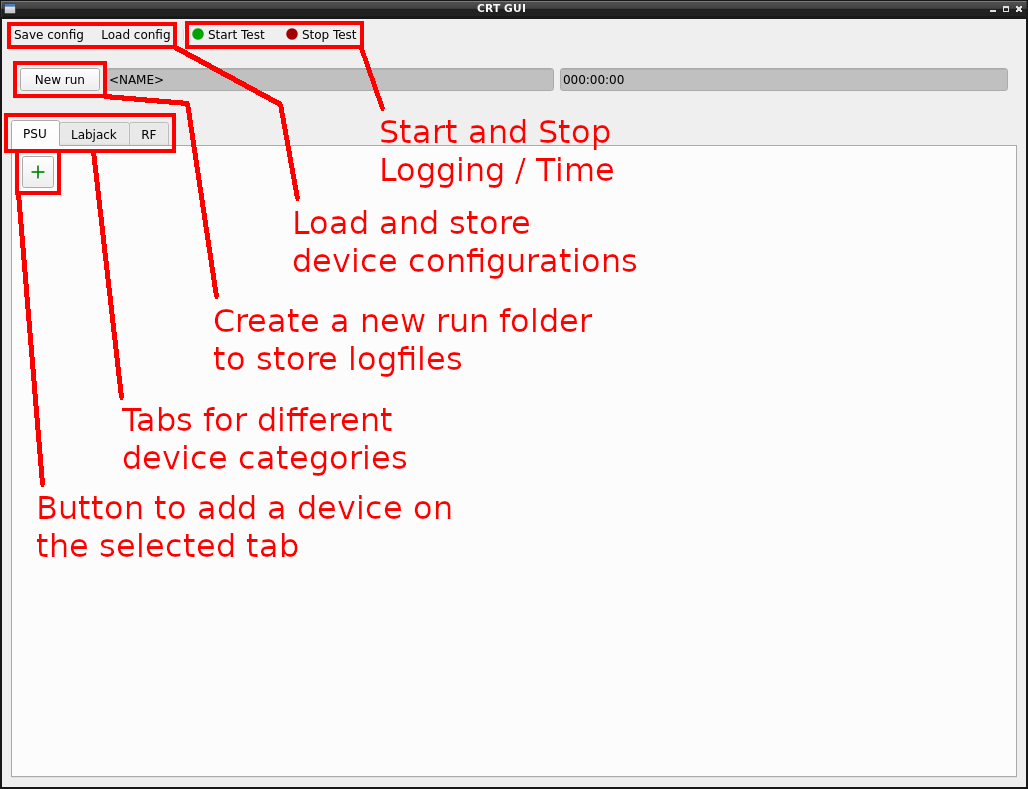
\includegraphics[width=0.9\textwidth]{./1_Plain_Expl.png}
	\caption{Main menu of the suite}
	\end{figure}
	
	\subsubsection{Top Row}	
	
	On the top row, on the left side, configurations for all the components in the various tabs can be either stored or loaded. The stored configuration file is also human readable and editable.
	
	\bigbreak
	
	On the right side the test can be started or stopped. Starting and stopping the test sends a trigger to all components. E.g. the power supply will turn selected channels on/off and start/stop the logging. Hence one can not click the start-button twice in a row!
	
	\subsubsection{Run Information (Mid Row)}
	
	In the row below is the run information. To start a run one should first create a \enquote{New run} by clicking the button and creating a folder to store all the log files. On the right of this button, the current file location and the time of the run are displayed. If one stops the run, the time also halts till the run gets restarted. 

	\bigbreak	
	
	The log files are named after the individual components, so one should make sure to not have any names twice.
	
	\subsubsection{Tabs}
	
	The tabs contain various devices of the same kind. Currently implemented are:
	
	\begin{itemize}
	\item Power-supply
	\item Labjack
	\item RF (Reception client for the Analog Devices IIO-daemon)
	\end{itemize}		
	
	\subsection{Testrun}	
	
	\begin{figure}[H]
	\centering
	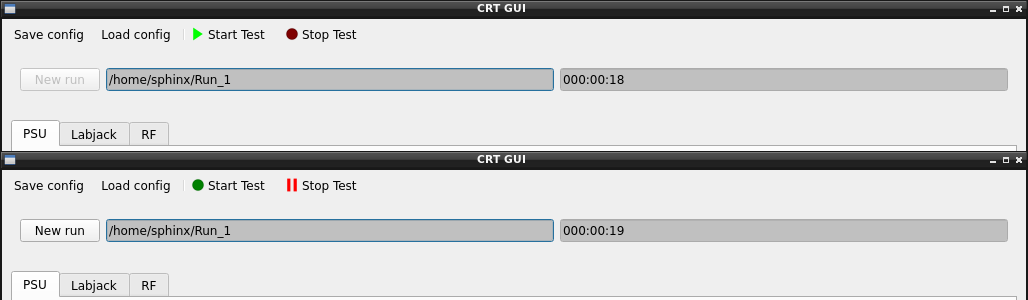
\includegraphics[width=0.9\textwidth]{./4_Testrun.png}
	\caption{An active testrun in the suite}
	\end{figure}
	
	If a test run is started, the \enquote{Start} button and the \enquote{New run} button get deactivated and the time starts to count up. Meanwhile in the background, logfiles are generated with a UTC timestamp. The data itself is stored in a \textit{.csv} format to be easily readable. To every datapoint or row being stored, a relative timestamp in milliseconds is added.
	
	\bigbreak
	
	To stop the run and therefore also the logging and timer, the \enquote{Stop} button should be pressed. After that a run can also be continued by clicking the \enquote{Start} button again.	
	
\section{Components}

	\subsection{Power-Supply}
	
	\begin{figure}[H]
	\centering
	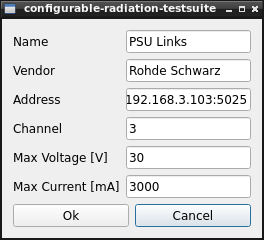
\includegraphics[width=0.4\textwidth]{./2_PSU_menu.png}
	\caption{An active testrun in the suite}
	\label{f:psu_menu}
	\end{figure}
	
	The power supply can be either added via configuration file or manually. If it's added manually a small window will pop up (see figure \ref{f:psu_menu}). 
	
	\subsubsection{Manual Creation}	
	\label{c:psu_manual_creation}
	
	The window for manual creation is presented in figure \ref{f:psu_menu}. In the first row an individual (meaningful) name can be chosen. In the second row the vendor is put in (case insensitive). Then follows the address which has a IPv4 part and a port number after the double dot. In the last three rows a description of the power supply is given with the number of channels and the maximum voltage / current the supply has or one wants to apply.	
	
	\subsubsection{Config Creation}
	
	The power-supply is denoted in the configuration file in the \enquote{PSU} section. The first four lines correspond to the manual creation in chapter \ref{c:psu_manual_creation}. After that the current channel settings are brought up. They have a prefix $c$, a number $X$ as identifier and a suffix $v$ for voltage and $c$ for current.
	
	\begin{lstlisting}
	Section PSU
		name=PSU Links
		address=192.168.3.103:5025
		channel=3
		max_voltage=30
		max_current=10
		c0v=10
		c0c=3
		c1v=10
		c1c=3
		c2v=10
		c2c=3
		signal=
	EndSection
	\end{lstlisting}
	
		\subsubsection{Supported devices}
		Support for other devices can be easily added. One only needs to edit the \textit{psu.*} files and add a few lines for the correct SCPI\footnote{Standard Commands for Programmable Instruments} Code.
	
		\begin{table}[H]
		\centering
		\begin{tabular}{ll}
		\toprule
		Supplier			& Model \\ \midrule
		Rhode\&Schwarz		& HMC8043 \\
		TTI					& (?) \\
		\bottomrule
		\end{tabular}			
		\end{table}	
	
	\subsection{Labjack}
	
	\begin{figure}[H]
	\centering
	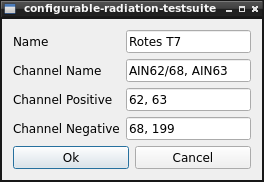
\includegraphics[width=0.4\textwidth]{./3_LBJ_menu.png}
	\caption{An active testrun in the suite}
	\label{f:lbj_menu}
	\end{figure}
	
	The labjack can be either added via configuration file or manually. If it's added manually a small window will pop up (see figure \ref{f:lbj_menu}).
	
	\subsubsection{Manual Creation}	
	
	The window for manual creation is presented in figure \ref{f:lbj_menu}. In the first row an individual name can be chosen. The channel names in the second row can also be chosen individually. The third and fourth row determines the used channels\footnote{Refer to \url{labjack.com/support/datasheets/t-series/ain}} and if they are differential or not. A differential channel is given by a certain positive and negative address, whereas single ended just use $199$ as negative channel.
	
	\subsubsection{Config Creation}	
	The power-supply is denoted in the configuration file in the \enquote{PSU} section. First the name is defined and after that the number of channels as a validity check. The individual channels are written with a prefix $c$, a number $X$ and their features as prefix:
	
	\begin{itemize}
	\item $n$: Name
	\item $pc$: Positive Channel
	\item $nc$: Negative Channel
	\item $b$: Boundary value
	\item $g$: Gain value
	\end{itemize}
	
	\begin{lstlisting}
	Section LBJ
		name=Rotes T7
		channel=2
		c0n=AIN62/68
		c0pc=62
		c0nc=68
		c0b=0
		c0g=1
		c1n=AIN63
		c1pc=63
		c1nc=199
		c1b=0
		c1g=1
		signal=
	EndSection
	\end{lstlisting}
	
		\subsubsection{Supported devices}
		To support other devices the addresses in the \textit{Labjack.*} files have to be extended.
	
		\begin{table}[H]
		\centering
		\begin{tabular}{ll}
		\toprule
		Supplier			& Model \\ \midrule
		Labjack				& T7 \\
		\bottomrule
		\end{tabular}			
		\end{table}	

	\subsection{RF Signals}
	Not implemented yet
	
		\subsubsection{IIO Daemon}
		
	\subsection{Ethernet}
	Not implemented yet

\appendix

\section{Diagrams}

	

\end{document}